\documentclass[applsci,article,accept,moreauthors,pdftex]{Definitions/mdpi}

\usepackage{gensymb}
\usepackage{placeins} % gives the command \FloatBarrier, which will make sure any floats will be put in before this point
\usepackage{flafter}  % ensures that floats don't appear until after they appear in the code.
\usepackage{dblfloatfix} % Try to place figure spanning the whole width (figure* envs) in tbp
%\usepackage{subcaption} % to have two figures side-by-side
\usepackage{subfigure}
\makeatletter
\renewcommand{\@thesubfigure}{\normalsize(\textbf{\alph{subfigure}})}
\makeatother

%=================================================================
% Full title of the paper (Capitalized)
\Title{Simpler Learning of Robotic Manipulation of Clothing by Utilizing DIY Smart Textile Technology}

\abstract{Deformable objects such as ropes, wires, and clothing are omnipresent in society and industry but are little researched in robotics research. This is due to the infinite amount of possible state configurations caused by the deformations of the deformable object. Engineered approaches try to cope with this by implementing highly complex operations in order to estimate the state of the deformable object. This complexity can be circumvented by utilizing learning-based approaches, such as reinforcement learning, which can deal with the intrinsic high-dimensional state space of deformable objects. However, the reward function in reinforcement learning needs to measure the state configuration of the highly deformable object. Vision-based reward functions are difficult to implement, given the high dimensionality of the state and complex dynamic behavior. In this work, we propose the consideration of concepts beyond vision and incorporate other modalities which can be extracted from deformable objects. By integrating tactile sensor cells into a textile piece, proprioceptive capabilities are gained that are valuable as they provide a reward function to a reinforcement learning agent. We~demonstrate on a low-cost dual robotic arm setup that a physical agent can learn on a single CPU core to fold a rectangular patch of textile in the real world based on a learned reward function from tactile information.}

% Keywords
\keyword{deformable object manipulation; smart textile; low-cost; reinforcement learning}

\begin{document}

%===============================================================================
% COPY PASTE OK
\section{Introduction}
Industry and society benefit greatly from autonomous robots that are able to perform manipulation skills on complex objects. Recent work shows that it is possible to learn grasping~\cite{Levine2018, morrison2018cartman} and manipulation~\cite{Agrawal2016, Gu2017} skills on everyday objects. Although prior work has been undertaken~\cite{Levine2018} including deformable objects in the set of daily household objects, most robotic manipulation tasks are limited to objects with considerable stiffness, such as rubber ducks. Highly deformable objects---for example, cables or clothes---are often left out of the set due to the many challenges associated with handling the infinite amount of configurations these objects can be in~\cite{Foresti2004}.

Prior work~\cite{Saha2007, Maitin2010, Doumanoglou2016} has focused on scripting solutions for the robotic manipulation of deformable objects. However, the engineering effort to make this work is considerable, and the designed solutions often break down when the environment changes. Recent work~\cite{Matas2018, Seita2018} has leveraged learning methods that are able to generalize to a wider range of deformable objects. Often, these methods require the definition of the task in simulation in order to generate rollouts in the environment. Unfortunately, simulating cloth is both challenging and computationally expensive. Furthermore, there is no guarantee that the acquired skills in simulation are transferable to the real world. \par

A typical approach for the robotic folding of textile relies on the use of vision in order to detect grasping points and to perform texture segmentation and pose estimation~\cite{Maitin2010, Doumanoglou2016, Bersch2011}, as well to estimate the state~\cite{Matas2018} and---in the case of reinforcement learning (RL)-based approaches---the reward function~\cite{Tsurumine2019}. However, while~vision is instrumental for recognizing and localizing objects, touch and force measurements become important once contact occurs, and the object is explored using the end-effector~\cite{Billard2019}. Recent~work~\cite{Tian2019} has illustrated this idea by applying a touch-based control method for a ball repositioning task, rolling a dice and the deflection of a stick. In line with other authors~\cite{Tian2019, Lee2019}, we believe the use of tactile input and its fusion with other sensory information is crucial to learn complex robot manipulation tasks in an efficient way. \par

In this work, we deviate from the wider focus on using vision for state and pose estimation. Instead, we propose a cost-effective solution for the robotic folding of textile. Our approach is based on the use of the reinforcement learning of a shallow neural controller for a low-cost setup of a dual robotic arm, visible in Figure~\ref{fig:setup_overview}. Instead of engineering the reward function, we developed a smart textile piece that is able to detect whether it has been folded.
\begin{figure}[H]
\centering
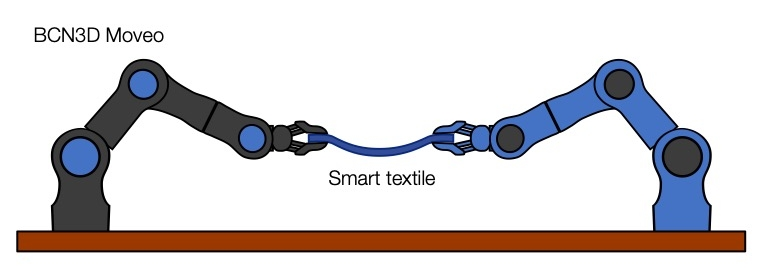
\includegraphics[width=0.9\textwidth, keepaspectratio]{figs/folding_overview_smaller.jpg}
\caption{Schematic overview of the setup: dual robot arms hold a smart textile piece and have to learn to fold it from scratch using sensory feedback of the textile and proprioceptive input of the robotic~arms. }
\label{fig:setup_overview}
\end{figure}


%===============================================================================

\section{Related Work}

\label{sec:related_work}

%! THIS SECTION WAT NOT COPY PASTED

% ---- Cloth manipulation pipelines
When calculating the required trajectories for deformable object manipulation, the deformations need to be taken into account~\cite{Foresti2004}. One approach to incorporating this is by using simulation. In~\cite{Yamakawa2011}, for example, deformations of a linear flexible object are approximated in a simulation in order to generate trajectories for folding in the air. In the case of clothing, the prior work presented in ~\cite{Maitin2010,Doumanoglou2016} dealt with the high-dimensional clothing state by building folding processes in which grasping points are manually chosen so that wrinkles are minimized. Next, the executed manipulation trajectories are hard-coded or calculated by matching polygonal models to contours. However, these approaches can accumulate errors across stages. For example, the type of textile can be mislabelled early in the process, leading to subsequent incorrect pipeline operations~\cite{Doumanoglou2016}. Additionally, engineered robotic pipelines for the folding task can take up to 24 min to execute~\cite{Maitin2010}, with the grasp point detection phase being the largest bottleneck. In~\cite{Willimon2011}, a faster process was implemented which could grasp and classify clothing in one minute. There were two overhead cameras in their setup, but the view was occluded when the arm engages. Consequently, the grasping procedure had to be executed repeatedly at different heights in order to detect whether an isolated garment was grasped.\par

% ---- Deep RL for textile manipulation
To avoid highly-engineered pipelines and the associated loss of information between the stages, more recent methods utilize learning methods in order to grasp or manipulate deformable objects. For~example, in \cite{Matas2018}, deep reinforcement learning is used to train a neural network to learn to manipulate a towel. The controller is trained in simulation and transferred to the real platform using domain randomization. In their approach, the agent learns from the pixel input only, while our method leverages tactile sensing to attain a more informational representation of the cloth. In~\cite{Arnold2019}, a forward dynamics model of the cloth using a latent space representation is learned. This architecture is used in~\cite{Tanaka2018} to bring cloth into the desired configuration. However, transferring this to the real world is challenging due to the difficulty in generating high-fidelity rollouts in simulation~\cite{Matas2018, Tanaka2018}. In our work, the policy of the robot is learned to avoid sim-to-real transfer issues. Other work tries to overcome the many training demonstrations required for training by utilizing learning from demonstration methods in order to speed up the training process~\cite{Balaguer2011, Laskey2017}. This was illustrated in~\cite{Rahmatizadeh2018}, who used teleoperated demonstrations to teach a low-cost robotic setup multiple tasks. However, general-purpose, dual-armed robots typically contain many degrees of freedom (e.g.,~the humanoid dual-arm Baxter\textsuperscript{\textregistered} robot contains seven degrees of freedom per arm~\cite{Baxter}), making teleoperation~difficult.\par

% ---- reward function for learning cloth manipulation
Defining a reward function for the robotic folding task is difficult because it requires the state estimation of the cloth. Previous work~\cite{Doumanoglou2016,Miller2012} has extracted the contour of the textile using color segmentation. In~\cite{Balaguer2011}, a marked towel is tracked, allowing the calculation of the distance between points on the towel from the training sample and the example demonstrations so that it can be used as a reward for the agent. Their method requires prior information about the shape of the object in order to reconstruct the missing market points. More recent work in using (deep) reinforcement learning for robotic folding also used vision-based methods to define the reward function for the agent~\cite{Tsurumine2019, Matas2018}. However, relying~solely on visual inputs and marker clues does not scale well. Another approach to find a reward function was explored in~\cite{Abbeel2004, Finn2016}, where inverse reinforcement learning (IRL) was used to learn a reward function from expert demonstrations. Because IRL learns a reward function and a policy separately, it~requires RL to be run in an inner loop, making it computationally expensive to train. Our~approach learns the reward function offline in a supervised way, making it feasible to train on a real~robot.


%===============================================================================
\section{Learning to Fold Textile with Low-Cost Hardware}
\label{sec:setup}
In this work, we propose a shallow neural network controller that is able to learn control policies for a dual-arm robot using reinforcement learning with the aim of folding a textile piece. An overview of our setup is given in Figure~\ref{fig:setup_overview}.

\subsection{An Inexpensive Setup for Textile Folding}
% ! COPY PASTED
\label{subsec:robots}
Our setup consists of two robot arms that have to fold a piece of textile. In order to demonstrate the possibility of applying our methodology in a low-cost setting, we constructed the BCN3D Moveo robot arms (\url{https://github.com/BCN3D/BCN3D-Moveo}). These robot arms have five degrees of freedom each and are low-cost and open source. They can be fabricated by rapid prototyping techniques and off-the-shelf components. The textile piece was attached to the grippers by means of a hook-and-loop~fastener.

\subsection{Fitted Q-Learning}
\label{subsec:rl}
% ! COPY PASTED

In order to train a controller for robotic folding, we use fitted Q-learning~\cite{Watkins1992}, a model-free reinforcement learning method in which the expected discounted reward of state--action pairs are calculated based on rollouts in the environment. We utilize experience replay~\cite{Lin1992} and approximate the Q-function with a shallow multilayer perceptron (MLP). We define a sparse reward function that gives a large reward upon folding the cloth. However, this requires the detection of the state of the cloth---a~non-trivial task given the high amount of cloth configurations. Hand-engineered heuristics to estimate the cloth state have been researched~\cite{Doumanoglou2016} but are highly complex to reproduce and are prone to error. Visual cues such as colored surfaces or fiducial markers~\cite{Bersch2011, Tsurumine2019} can be attached to highly deformable materials but require the many occlusions caused by the self-collision of the cloth to be~handled.

% =================================================
\section{Smart Textile}
% ! COPY PASTED
\label{sec:textile}

In order to solve the problems associated with using vision for the state estimation of cloth, we~developed an accessible, low-cost smart textile that can identify its actual pose. By integrating a flexible tactile sensor grid into a flat textile piece, a pose estimation model can be trained. Consequently, the~textile is able to sense and react to its surrounding environment, making it self-aware or making it an active smart textile~\cite{Stoppa2014}.

The layers in the smart textile can be seen in Figure~\ref{fig:textile_scheme}. The textile consists of piezoresistive rubber (commercially available as Velostat\textsuperscript{\textregistered}) that is sandwiched between two layers of conductive threads that act as electrodes~\cite{Drimus2014}. The electrodes are made of copper strips that are insulated with a polyimide film. This results in a matrix of $12$ by $7$ tactile cells. The signal conditioning for measuring the pressure applied over a tactile cell is based on the voltage divider principle. More specifically, the~voltage is measured between the tactile cell, which acts as a variable resistor, and a fixed resistor of $5.6$~kOhm. The voltage was measured and processed by a standard microcontroller. The resulting textile can be seen in Figure~\ref{fig:textile_real}.

Based on the output of the $12$ by $7$ tactile cells, a linear classifier is trained to predict the garment state: folded or unfolded. Therefore, we first collected data from the tactile cells by bringing the cloth into multiple configurations while hand-labelling the associated state. We define the folded state of the cloth with some slack because of the way in which the robots are positioned in order to avoid a collision; this is illustrated in Figure~\ref{fig:folded_real}. The collected data were split into a training set of $1418$ samples and a test set of $511$ samples. In Figure~\ref{fig:sensor_data}, the average voltage and standard deviation of the tactile cells for both garment states are shown. One can observe that there is a clear voltage peak in the center column, implying that the tactile cells in the center of the textile experience higher pressure due to the folded~state.
\begin{figure}[H]
\centering
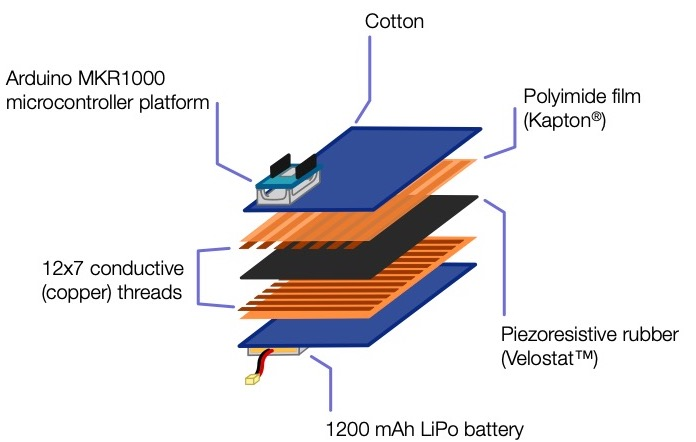
\includegraphics[width=0.85\textwidth, keepaspectratio]{figs/textile_overview.jpg}
\caption{Exploded-view drawing of the textile with integrated tactile sensing. Conductive threads organized in a $12$ by $7$ grid are applied on piezoresistive rubber, creating a variable resistor. The~resulting voltage acts as a proxy for local forces applied on the cloth. } %Please define MKR if appropriate.
\label{fig:textile_scheme}
\end{figure}
\unskip

\begin{figure}[H]
\centering
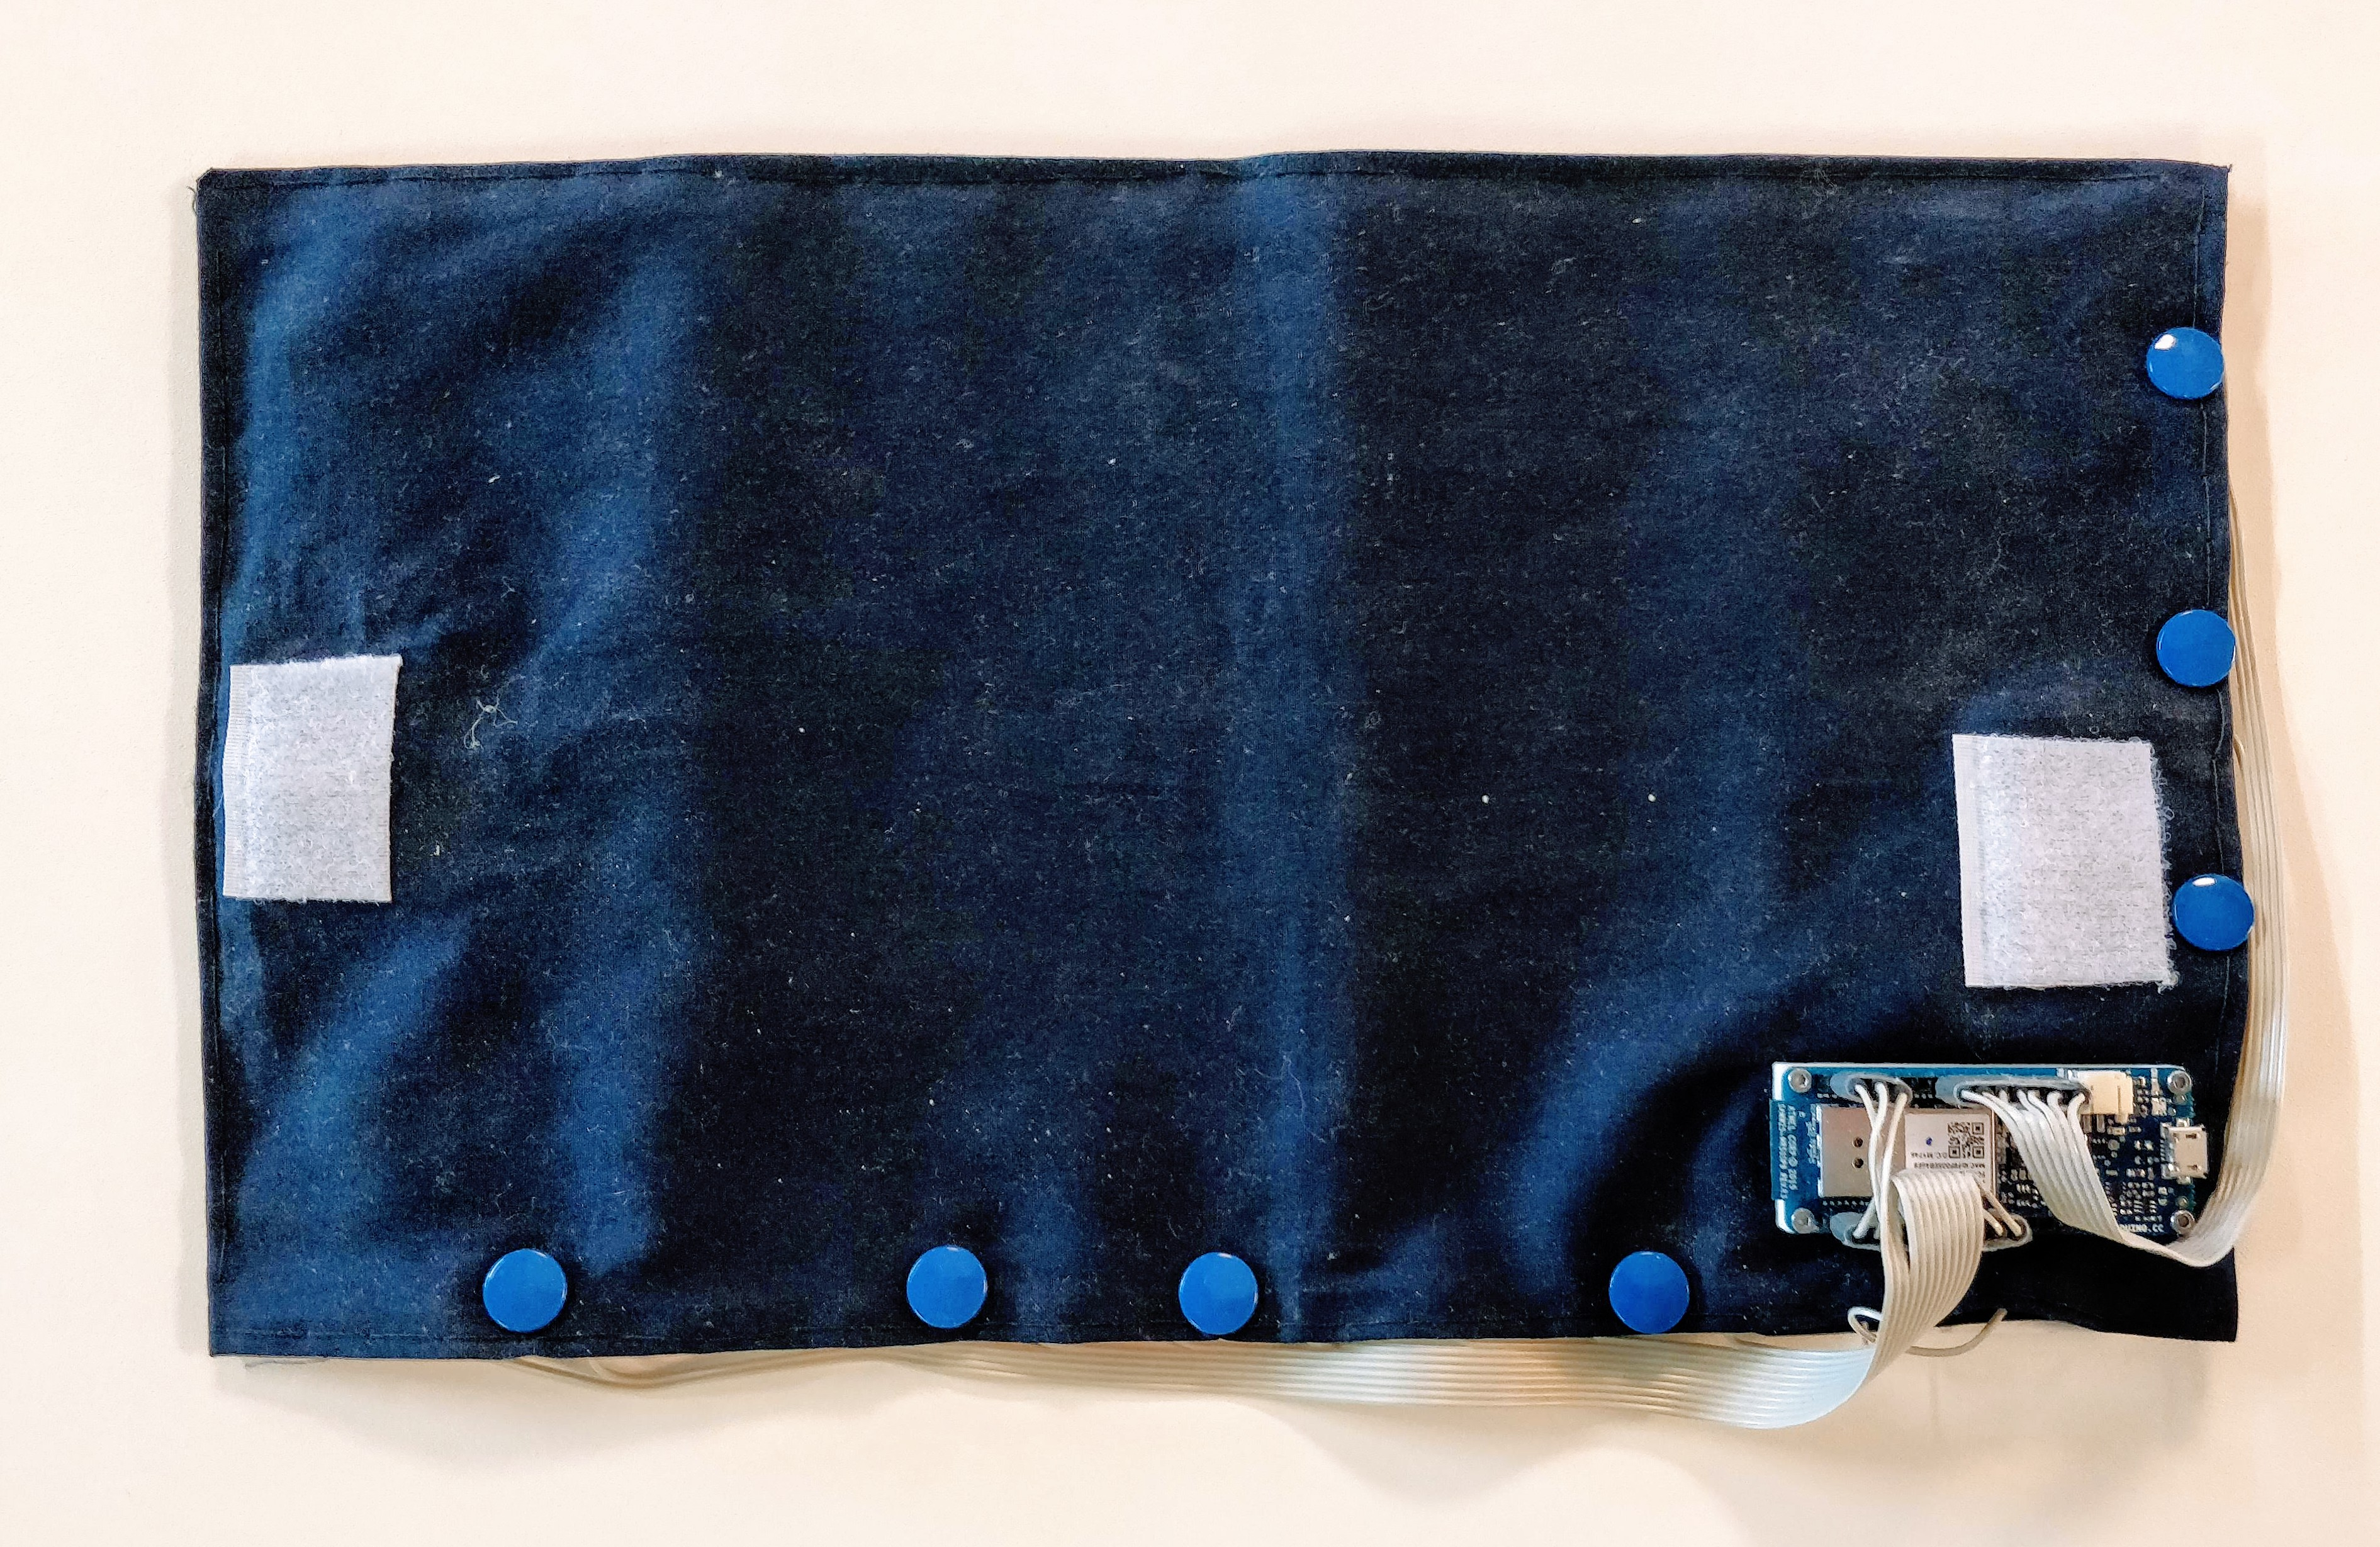
\includegraphics[width=0.90\textwidth, keepaspectratio]{figs/textile.jpg}
\caption{Our resulting implementation of a smart textile which is able to detect and translate local forces to a state configuration (for example, folded or unfolded). The smart textile is made using accessible off-the-shelf materials and tools.}
\label{fig:textile_real}
\end{figure}
\unskip

\begin{figure}[H]
\centering
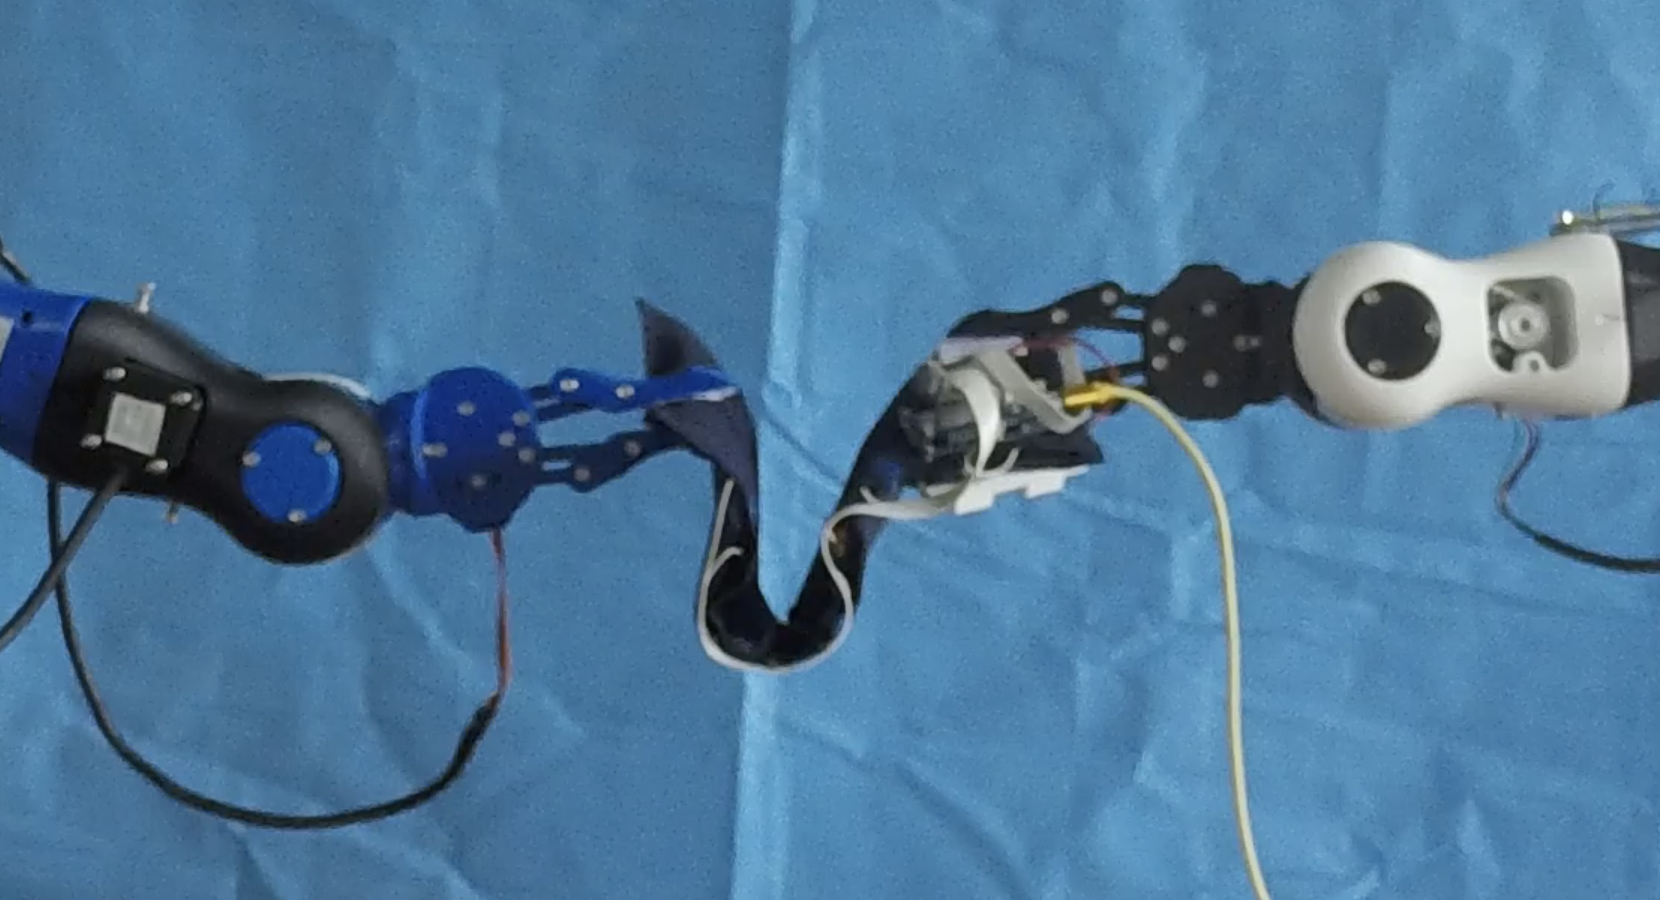
\includegraphics[width=0.90\textwidth, keepaspectratio]{figs/folded_real.png}
\caption{Example of the folding task on the real platform. The robotic arms are positioned in such a way that they cannot collide, making it physically impossible to fold the cloth fully. Thus, we do not require a fully folded state of the textile from the agent.}
\label{fig:folded_real}
\end{figure}
\unskip

\begin{figure}[H]
\centering
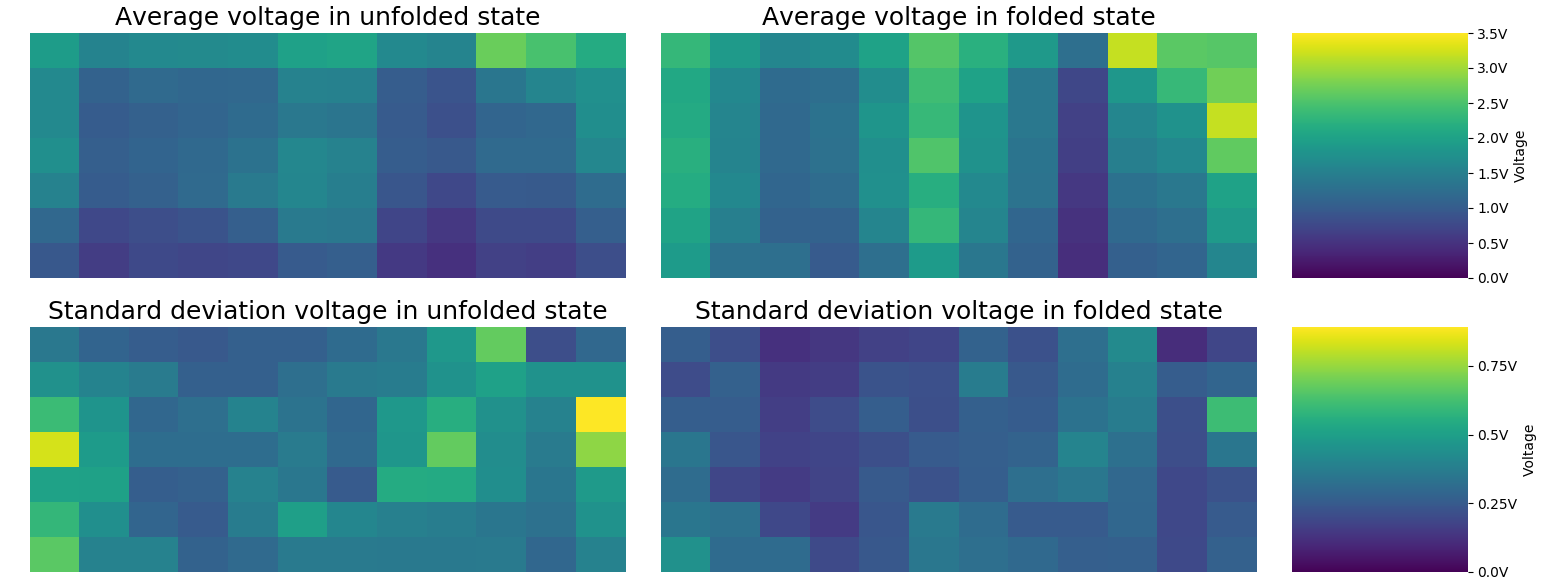
\includegraphics[width=\textwidth, keepaspectratio]{figs/sensor_data_over_states.png}
\caption{The average and standard\textls[-15]{ deviation of the collected data from the 12 by 7 tactile cells show a higher voltage in the center column---where the fold is---when the cloth is in the folded state. These~figures qualitatively indicate that the tactile cells in the textile react to different folding configurations}. }
\label{fig:sensor_data}
\end{figure}

The classifier was trained using logistic regression with l2-norm regularization on 1418 training samples in a five-fold cross-validation setting. The regularization parameter was optimized by performing a random search and by using the F1-score as a performance metric. In order to verify the usability of the classifier, we tested it on an unseen test set of 511 samples which resulted in an average F1-score of $0.97$. The full results of the test set are summarized in Table~\ref{table:classifier_results}.
\begin{table}[H]
\centering
\caption{\textls[-15]{Test set results of the linear classifier that \textls[-15]{detects whether the cloth has been folded (511 samples).} The high classification performance means that the smart textile is suitable to be used as a reward function}.}
\label{table:classifier_results}
\begin{tabular}{ccccc}
\toprule
& \textbf{Samples} & \textbf{Precision} & \textbf{Recall} & \textbf{f1-Score} \\
\midrule
Unfolded &  342 &     0.98    &  0.98  &    0.98 \\
Folded & 169  &       0.96  & 0.95  &    0.96 \\
\bottomrule
\end{tabular}
\end{table}


We are able to classify different shape configurations for the textile piece with high accuracy, making the smart textile useful for learning purposes. Other desired features such as wrinkle detection are hard to measure with this technology given the limited sensitivity of the piezoresistive rubber~used.


%===============================================================================
% ! COPY PASTED
\section{Results}
\label{sec:results}

As described in Section~\ref{sec:setup}, the task consists of folding a rectangular textile piece by using a low-cost dual robotic arm. The arms are positioned in an opposing manner to avoid a collision. In order to avoid damaging the smart textile, we limited the movement of each robot arm to three degrees of freedom~(DOF) instead of the available five~DOF. Consequently, the movements of the robots are limited to one plane.

In order to find the control policy for folding, we formulated the problem as a fitted Q-learning problem. The state-space $S=\mathbb{R}^6$ is defined by the joint space of the dual-arm robot, with six motor angels in total. For each joint, we define two actions: $\pm \Delta$ with $\Delta$ equal to $4 \degree$. The reward function $R$ is sparse and defined by
\begin{equation*}
R=
\begin{cases}
100 & \text{on success} \\
-1  & \text{penalty for wandering}
\end{cases}
\end{equation*}

We approximate the Q-function with a simple MLP with six input neurons (one for each of the controlled joints), two hidden layers with  $128$ and $64$ ReLu neurons, respectively, and $12$ output (linear) neurons (one for each of the possible actions). In order to find a good set of parameters, we implemented a simple forward kinematic model of the robot arms in a reaching task setting. This~allowed us to sweep across various hyperparameter settings. The optimizer we used is stochastic gradient descent with a learning rate of $0.01$ and batch size of $64$ samples. The target network is updated each $1000$ steps. Exploration is done using an $\epsilon$-softmax policy with $5000$ exploration steps. Thus, the agent will first execute fully random motor actions and gradually start choosing actions that maximize the expected q-values.

After the selection of the hyperparameters, we trained our dual robotic arm setup from scratch in the real world. As shown in Figure~\ref{fig:results}a, after approximately $60$ episodes (17,000 steps, or $8$ h), the robot successfully learned to complete the folding task. Figure~\ref{fig:results}b shows the number of steps the robot needs to fold the cloth per episode. The low dimensional state space of the agent and the learned reward function from tactile information using supervised learning allows the agent to learn to fold the cloth after relatively few training examples.

An example trajectory of the learned policy is shown in Figure~\ref{fig:robot_success_merge}. The action probabilities show that at the start of the episode, the agent primarily moves the shoulder joints, as they lead to the largest movement of the end-effector. This behavior has the benefit that it minimizes the penalty associated with wandering or other suboptimal movements. As the episode progresses, the agent has a higher probability of actuating the elbow and end-effector motors for more refined movement. The~end-effector trajectories, shown in yellow, are not smooth given that the policy is an action probability function calculated over the Q-values of the neural network. Because there are multiple reaching points in the plane to fold the cloth, the agent has multiple options to move during the first part of the episode, leading to jagged end-effector trajectories.

As our experiment illustrates, it is possible to avoid the need for complex vision-based state estimation to learn difficult tasks such as the folding of clothing with low-cost robots. The use of other input modalities such as a smart textile allows a reward function to be learned with simple linear models and is applicable to use for learning on real robotic platforms.
\begin{figure}[H]
\centering
\begin{tabular}{cc}
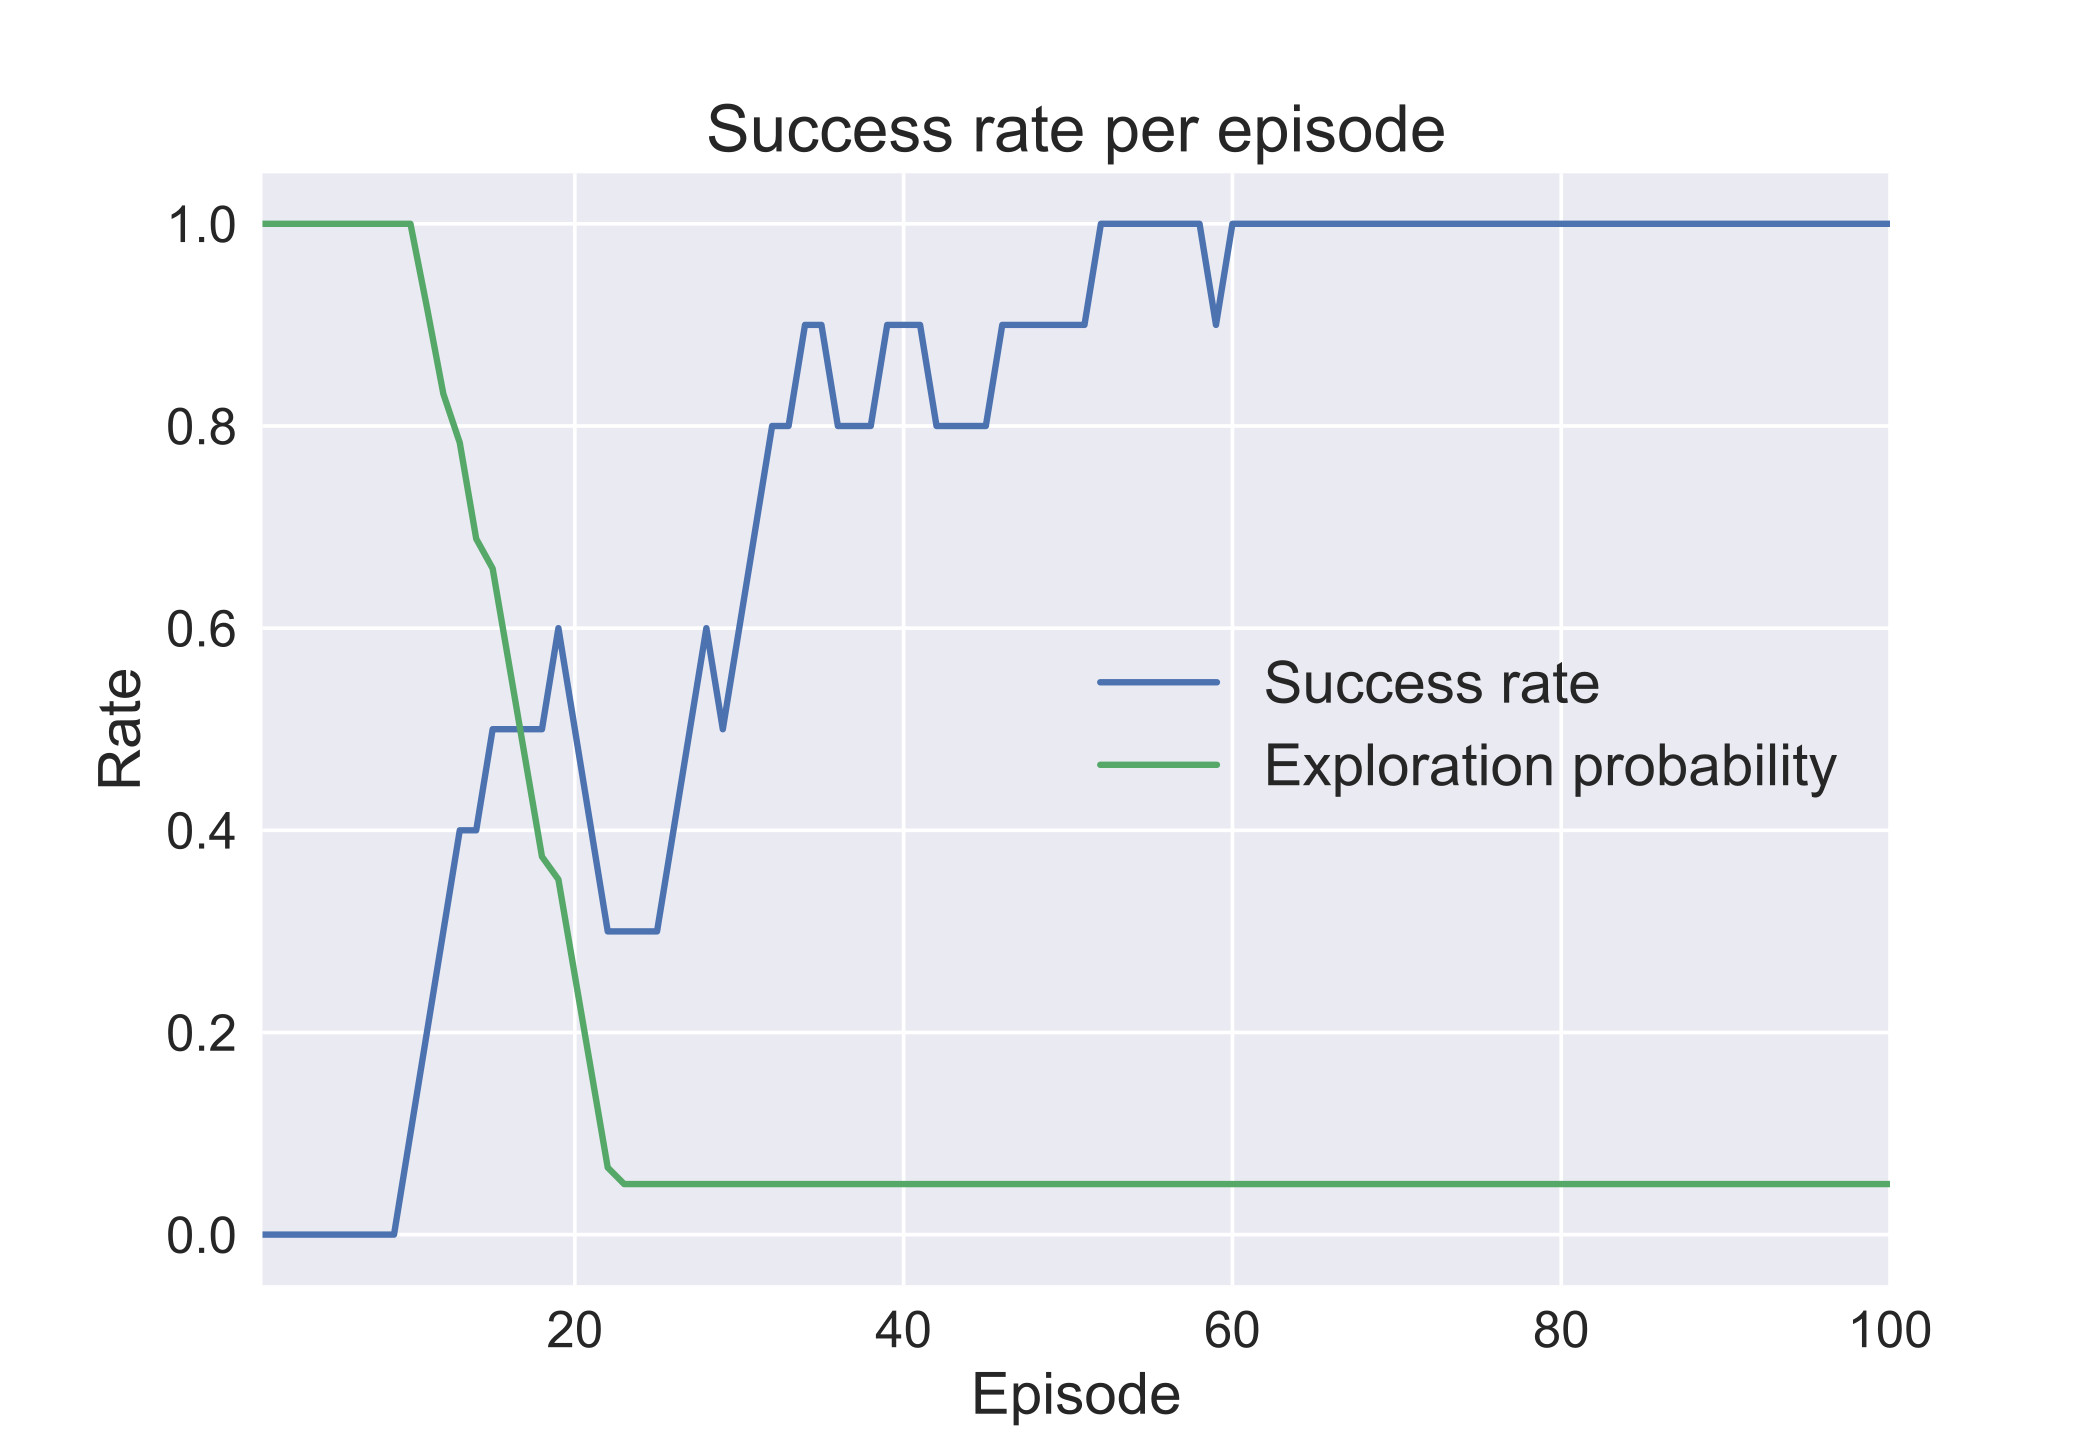
\includegraphics[width=0.48\linewidth]{figs/avg-success-rate.jpg}
&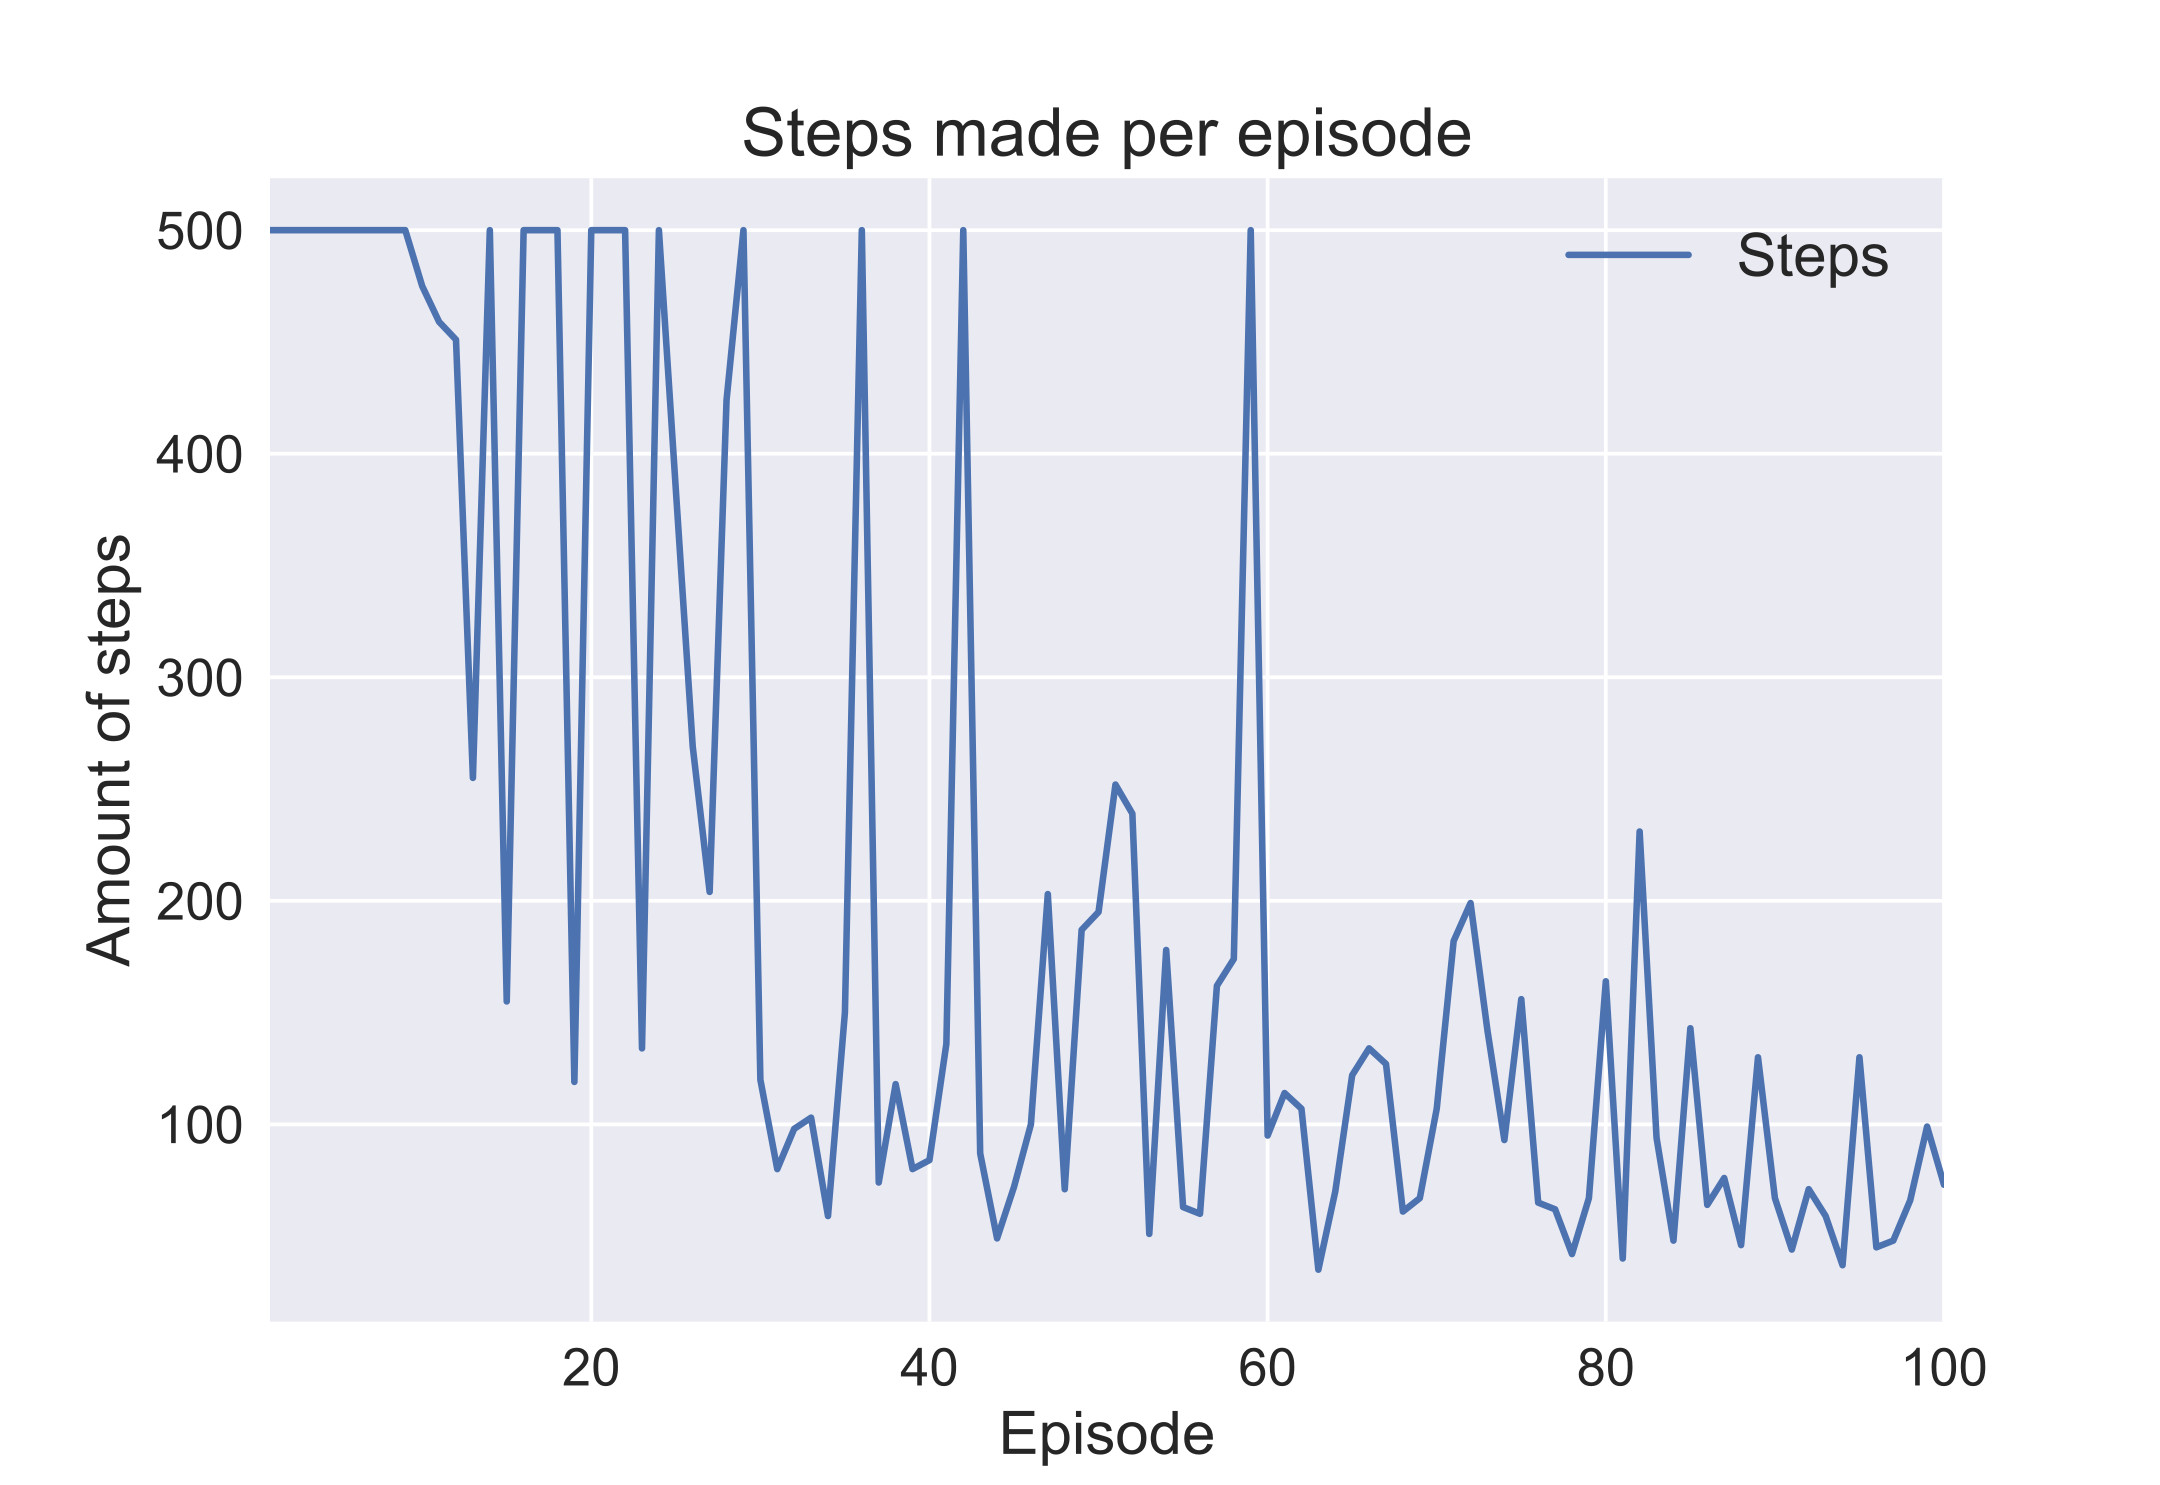
\includegraphics[width=0.48\linewidth]{figs/steps.jpg}\\
({\bf a})&({\bf b})\\
\end{tabular}
\caption{Results of training the real robot from scratch to learn how to fold a smart textile. (\textbf{a})~The~folding success rate and exploration probability per episode. \textls[-15]{The success rate grows to $100\%$ after training for $8$ h on the real robot. (\textbf{b})  The amount of steps required per episode to solve the task; the amount of motor commands needed to fold the cloth decreases after relatively few training examples}.}
\label{fig:results}
\end{figure}
\unskip

\begin{figure}[H]
\centering
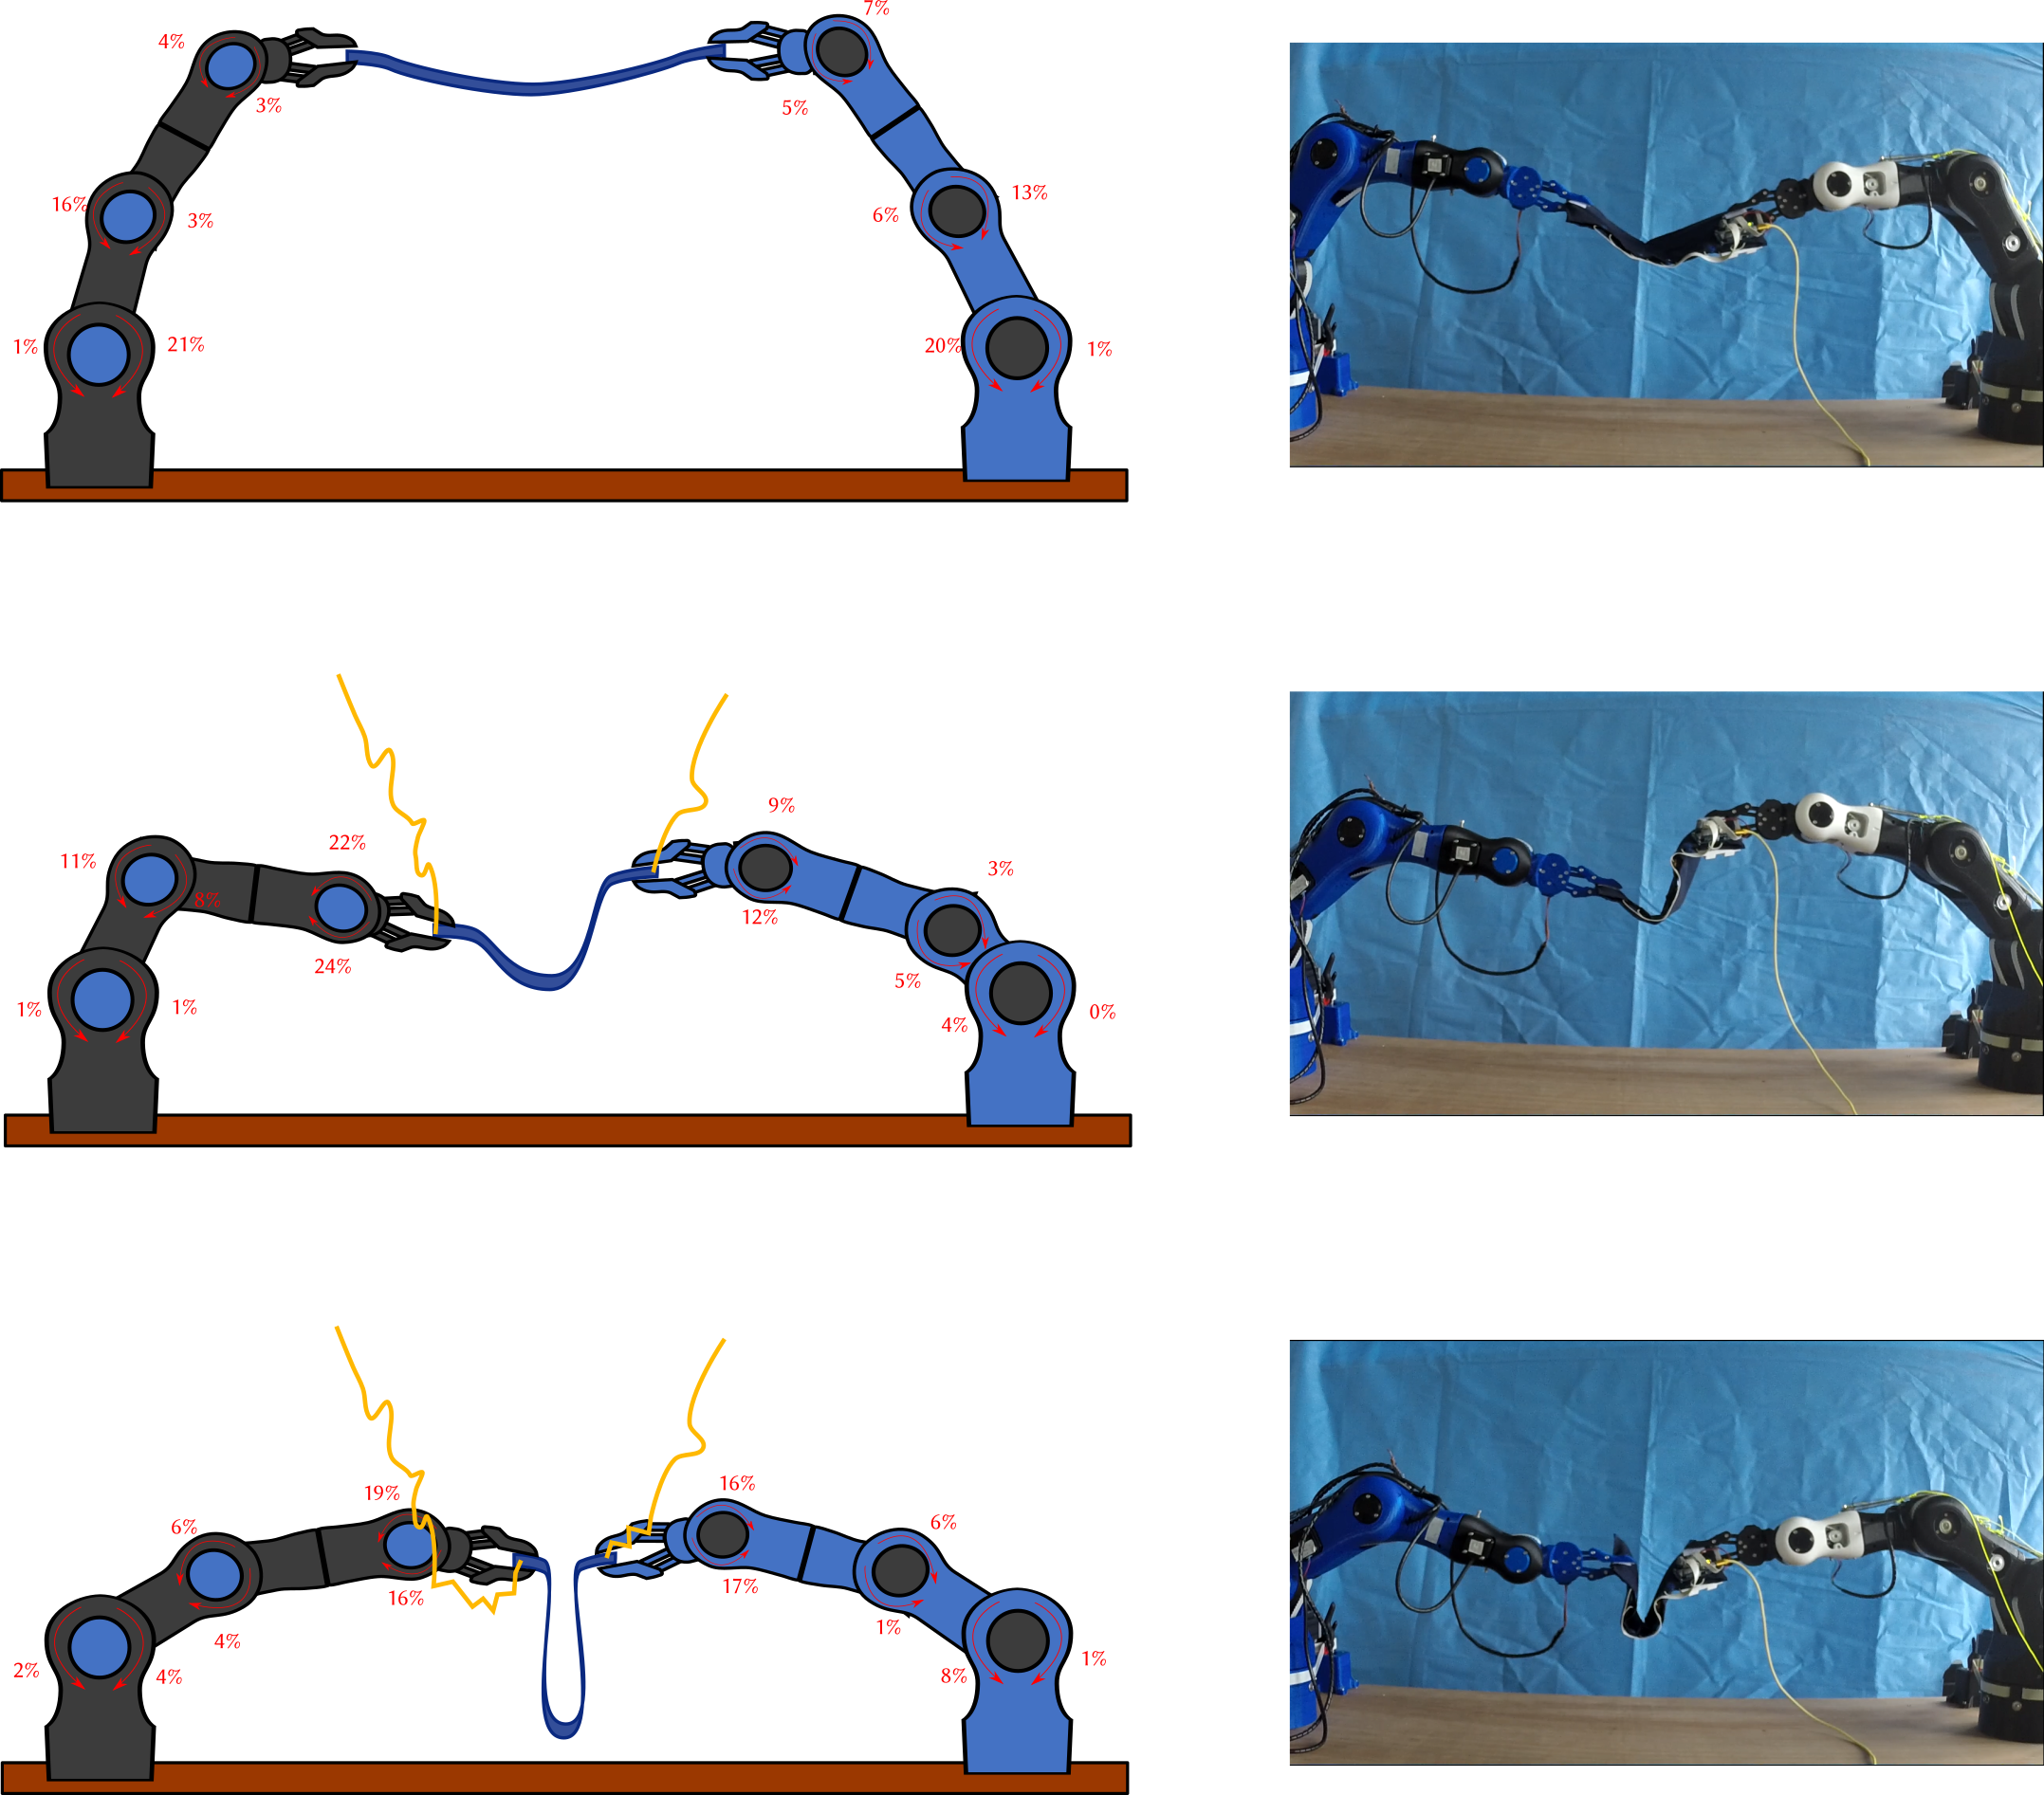
\includegraphics[width=0.9\textwidth, keepaspectratio]{figs/robot_success_merge_with_pics.png}
\caption{Demonstration of a folding trajectory of the learned policy broken down into three steps: start, middle and end of the episode. The robot state on the figure is visible from the stance of the robot arms. The action probabilities are given in red next to each joint. The executed trajectory is shown with a yellow line.  }
\label{fig:robot_success_merge}
\end{figure}
%===============================================================================

\FloatBarrier

% ! COPY PASTED
\section{Conclusions and Future Work} 
\label{sec:discussion}

Deformable objects are omnipresent in our daily environment and industry but little studied in deep reinforcement learning. In this paper, we proposed a cost-effective and computationally efficient solution for learning robotic manipulation skills for deformable objects. We have shown that an inexpensive dual robotic platform can learn to fold a textile piece in the real world with neural fitted Q-learning and without reward engineering. This is done by including tactile sensing in the learning process. We have shown that the high sensitivity of the proposed tactile cells allows the capture of arbitrary cloth configurations. We demonstrated that these tactile data can be used to train a simple logistic regression classifier to detect the cloth state; thus, we create a smart textile piece that is able to accurately detect whether it is folded.

The process proposed in this paper is feasible to scale up to other instances of cloth manipulation tasks given the low computational requirements and the tactile sensitivity of the sensor matrix. The~accessible fabrication procedure of the smart textile allows the implementation of this technology for any type of clothing, such as shirts and trousers. The influence on the deformable properties of the cloth can be reduced by miniaturizing the electronics, by using conductive thread instead of copper wires, and by only applying tactile cells in crucial areas. Future work includes exploiting the sensitivity of the tactile sensor grid to classify more complex cloth configurations and using more powerful, non-linear classifiers compared to the logistic regression model used in this work. Future research should be directed towards fusing the tactile information with visual data in order to generate a database of self-labeled images of arbitrary cloth configurations. These data can be produced by manipulating the cloth while recording its state with cameras. In order to detect and grasp the cloth and train policies that minimize wrinkles, visual feedback will have to be included. A suitable approach to integrate visual and tactile information is to learn a multimodal latent space, as shown in~\cite{Lee2019}.

We argue that by integrating a simple smart textile in the robot learning process, one can avoid the engineering of a reward function. In our approach, we avoided the use of vision for all steps in the learning process. Consequently, we can easily run the learning process in the real world using limited computational power. In our case, the state was purely based on the kinematics of the dual robot arms. We are aware that, in order to scale up our tasks to real clothing, we will have to integrate vision for the state estimation as well. Consequently, we do not advocate vision-free solutions, but we argue for an interdisciplinary approach in which vision, proprioception and tactile information is combined in order to find the simplest solution of state and reward function estimation.

%%%%%%%%%%%%%%%%%%%%%%%%%%%%%%%%%%%%%%%%%%
\end{document}

